\documentclass{article}
\usepackage{hyperref}
\usepackage{tikz}
\usetikzlibrary{arrows,intersections}
\usetikzlibrary{decorations.markings}

\usepackage{amsmath} % Required for \varPsi below

\hypersetup{
    colorlinks=true,
    linkcolor=blue,
    filecolor=magenta,      
    urlcolor=cyan,
}
\usepackage{graphicx}
\usepackage{float}
\usepackage{rotating}

\begin{document}

\title{Titanic - ML Project}
\author{Bogdanowicz Michal Kamil, Geraci Luca}

\maketitle

\begin{abstract}
Report of the project for the course of ML 2019/2020.
\break The models used are Logistic Regression, Neural networks, Decision trees, Random forests and Naive Bayes Classifier. Code and data can be found on \href{https://github.com/michalbogdanowicz/ML-Titanic-2020}{GitHub}. 
\end{abstract}


\section{Proposition}
The proposition is using a set of machine learning methods to predict the people that would survive the Titanic sinking of 15 April 1912.

The methods that have been used are:

\begin{enumerate}  
\item Logistic Regression
\item Neural Networks
\item Decision Trees and Random Forest
\item Naive Bayes Classifier
\end{enumerate}

\section{Data}
\subsection{Incomplete Data}

The Data proposed to the professor was incomplete. It heavily reduced the available data to perform the best practices for evaluating a model. The test and training were already separated and ground truth was missing. So the complete dataset has been taken from the internet. In addition the complete list of survivors can be found at the Wikipedia page \href{https://en.wikipedia.org/wiki/Passengers_of_the_RMS_Titanic}{here} (not a ML-friendly format).
This data sadly is used to cheat on the  \href{https://www.kaggle.com/c/titanic/leaderboard}{Kaggle competition}. Making it a quite infamous one.

\subsection{Data Format}

\begin{itemize}
\item Ticket class
\item Survival 
\item Name
\item Sex
\item Age in years
\item sibsp : number of siblings / spouses aboard the Titanic
\item parch : number of parents / children aboard the Titanic
\item Ticket number	
\item Fare
\item Cabin/s assigned
\item Port of Embarkation	
\item Rescue Boat
\item Body
\item Destination
\end{itemize}

\subsection{Additional info}
\textbf{Ticket class}: A proxy for socio-economic status (SES)\\
1st = Upper\\
2nd = Middle\\
3rd = Lower\\
\\
\textbf{Age}: Age is fractional if less than 1. If the age is estimated, is it in the form of xx.5
\\\\
\textbf{sibsp}: The dataset defines family relations in this way
Sibling = brother, sister, stepbrother, stepsister
Spouse = husband, wife (mistresses and fiancés were ignored)
\\\\
\textbf{parch}: The dataset defines family relations in this way
Parent = mother, father
Child = daughter, son, stepdaughter, stepson
Some children traveled only with a nanny, therefore parch=0 for them.


\subsection{Data Preparation}
The data cannot be used as it is. Here is the procedure used for the data preparetion. This follows mostly the data that the project was supposed to use at the begining.

\begin{itemize}
\item \textbf{Handling of NA values} : Age, fare and embarked have null values. For Age and fare the mean age has been used and for embarked the mode.
\item \textbf{Extraction of title and name deletion} : The title is extracted from the name. And the name feature is deleted as being mostly unique and being given arbitrarly by parents does not add anything to the model. An argument could be made that title is correlated witht the ticket class.  
\item \textbf{Elimination of cabin}: The amount of different cabins and the frequency of NA is such that it wold not add anything to the model. Additionally some people had multiple cabins.
\item \textbf{Elimination of Ticket}: The ticket is shared by people who embarked together. But a feature would need to be created for each ticket. This would mean more than 500 new features. And possibly lead to overfitting on training set. 
\item \textbf{Elimination of body}: Indicates the fact that the body has been found. This means that the person 100\% died. Removed as it simplified too much the problem. 
\item  \textbf{Elimination of Ticket Number}: The Ticket Number is eliminated because it would only make sense to use to connect people with the same ticket number. This would create c.a 700 different features. Since using it as a single feature would add nothing to the model.
\item \textbf{Elimination of Boat}: The boat is the the boat that the person has been rescued on. This would mean near 100\% survivability. This had been removed because it simplifies too much the problem. (e.g. logistical regression was giving  95\% accuracy and disregarded most of other features).
\item \textbf{Elimination of home.dest}: The destination would not have changed anything. Add would have added 386 new features to handle.
\item \textbf{Dummy variables}: Sex, Title, Embarked and pcClass need to have dummy variables. That is n-1 features for each feature, with a one-hot encoding. This is because there is no linear correlation between their values and they do not express magnitude. PcClass actually does express a better income in reverse order. But let us assume that 1st class are not inherently "greater" than 3rd class passengers.
\end{itemize}
\newpage
\section{Logistic Regression}
\subsection{Remark}

Since a most of the feature are binary their square result the same value. That means that elevating features which have only values 0 and 1 adds nothing to the model. Even more, it adds a fully correlated feature. Which has a negative impact on the model. Thus only non-binary features are added at a higher degree.
\\
\subsection{Procedure}

Procedure used for selecting the Logistic Regression model.

\begin{enumerate}  
\item The maximum polynomial was chosen by comparing the measures obtained with Cross Validation (CV) methodology. The data can be seen in (Table
\ref{tab:LR-Measures}). Maximum degree 2 has prevailed in most iterations. At each iteration the folds are randomized, and maximum degree 1 rarely beat 2. 

\begin{table}[]
\centering
\caption{Polynomial degree measures comparison}
\label{tab:LR-Measures}
\begin{tabular}{|l|l|l|l|l|l|}
\hline
Measure/Degree  & 1     & \textbf{2}     & 3     & 4     & 5     \\ \hline
Accuracy  		& 0.804 & \textbf{0.810} & 0.717 & 0.662 & 0.437 \\ \hline
Precision		& 0.754 & \textbf{0.760} & 0.683 & 0.631 & 0.399 \\ \hline
Recall    		& 0.728 & \textbf{0.738} & 0.436 & 0.286 & 0.896 \\ \hline
F1        		& 0.738 & \textbf{0.746} & 0.515 & 0.390 & 0.534 \\ \hline
MAE       		& 0.196 & \textbf{0.190} & 0.283 & 0.338 & 0.563 \\ \hline
MSE       		& 0.196 & \textbf{0.190} & 0.283 & 0.338 & 0.563 \\ \hline
RAE       		& 0.414 & \textbf{0.403} & 0.599 & 0.715 & 1.193 \\ \hline
RSE       		& 0.828 & \textbf{0.806} & 1.197 & 1.430 & 2.385 \\ \hline
\end{tabular}
\end{table}

\item Bias and variance was checked by visualizing the Error in CV and Error on Training set on a graph with X as the degree of polynomial. As it can be seen in the (Graph \ref{Graph:LR-BV}), the cv and test MAE are very close. No Variance or Bias detected. 


\item Quality of the model was controlled with the construction of the learning curve in (Graph \ref{Graph:LR-LearningCurve}) to see if there was variance and more training samples were required. They were not, as the algorithm used in octave itself states around 200 iteration that the step become too small to be worth consideration.
\end{enumerate}


\begin{figure}
\centering
\begin{tikzpicture}[y=10cm, x=2.5cm]

% horizontal axis
\draw[->] (1,0) -- (5,0) node[anchor=north] {};
% labels
\draw	(1,0) node[anchor=north] {1}
		(2,0) node[anchor=north] {2}
		(3,0) node[anchor=north] {3}
		(4,0) node[anchor=north] {4}
		(5,0) node[anchor=north] {5};

\draw	(1,0.1) node[anchor=east] {0.1}
		(1,0.2) node[anchor=east] {0.2}
		(1,0.3) node[anchor=east] {0.3}
		(1,0.4) node[anchor=east] {0.4}
		(1,0.5) node[anchor=east] {0.5}
		(1,0.6) node[anchor=east] {0.6};

% vertical axis
\draw[->] (1,0) -- (1,0.7) node[anchor=east] {MAE};

% Error Training
\draw plot [smooth] coordinates {(1,0.18352)  (2,0.18029)  (3,0.27298)   (4,0.33461)  (5, 0.58153)};

\draw (2,0.140) node {$J(\theta )_t$}; %label

% Error CV
\draw plot [smooth] coordinates {(1,0.19481)  (2,0.19101)  (3,0.27659)   (4,0.33535)  (5, 0.57908)};
\draw (1.5,0.237) node {$J(\theta )_{cv}$}; %label

\end{tikzpicture}
\caption{Plot of Errors with CV and Training}
\label{Graph:LR-BV}
\end{figure}

\begin{figure}
\centering
\begin{tikzpicture}[y=10cm, x=0.05cm]

% horizontal axis
\draw[->] (1,0) -- (200,0) node[anchor=north] {};
% labels
\draw	(0,0) node[anchor=north] {0}
		(50,0) node[anchor=north] {50}
		(100,0) node[anchor=north] {100}
		(150,0) node[anchor=north] {150}
		(200,0) node[anchor=north] {200};

\draw	(1,0.1) node[anchor=east] {0.1}
		(1,0.2) node[anchor=east] {0.2}
		(1,0.3) node[anchor=east] {0.3}
		(1,0.4) node[anchor=east] {0.4}
		(1,0.5) node[anchor=east] {0.5}
		(1,0.6) node[anchor=east] {0.6};

% vertical axis
\draw[->] (1,0) -- (1,0.7) node[anchor=east] {MAE};

% Error Training
\draw (100,0.15) node {$J(\theta )_t$}; %label

\draw plot [smooth] coordinates {(5,0.61803)  (10,0.36619)  (25,0.34233)   (50,0.28343)  (100, 0.18589)(125, 0.18267)(135, 0.18216)(150, 0.18139)(190, 0.18088)};

% Error CV

\draw (100,0.260) node {$J(\theta )_{cv}$}; %label

\draw plot [smooth] coordinates {(5,0.61803)  (10,0.37738)  (25,0.34228)   (50,0.27804)  (100, 0.22609)(125, 0.18561)(135, 0.18868)(150, 0.18792)(190, 0.18867)};

\end{tikzpicture}
\caption{Logistic Regression Learning Curve for Max degree pol. = 2}
\label{Graph:LR-LearningCurve}

\end{figure}

\subsection{Chosen model.}
Every feature, with addition of the features not having only 0's and 1's elevated to the second power. With 400 max training samples ( default for octave, it would stop by himself having reached the limit around 200, when the adjustment step would be meaningless). 


\subsection{Outcome explanation}
The accuracy that has been reached is based on the ability of the logistic regression to use the correlation of the features to the survival of the person. It is more certain of a person's survival the more features with a positive weight are higher, and the more negative weighted features are lower . 
This can be seen by plotting the weights (which must then be related to the range of values taken by features). \\
The addition of squared features improving the accuracy means that there is a non-linear correlation between those features and the survival of a person. 
\newpage

\section{Neural Network}

\subsection{Procedure}

\begin{enumerate}
	\item The optimal, from the perspective of accuracy, number of nodes and the number of hidden layers has to be found. A CV based test battery has been set in order. It takes in consideration form 1 to 5 hidden layers and from 22 to 32 nodes per layer. As it can be seen in the table (Table \ref{tab:sklearn-NoScaling}) the best one has 2 hidden layers and 28 nodes per layer, achieves 0.813 accuracy. Do note that the chosen library already applies regularization.
	
	\item One feature that is provided by sklearn is scaling. i.e. data is scaled to have a mean of 0 and std of 1. The methods used are said to improve with the scaling. Another test battery was performed similar to step 1. This time with the feature added. The accuracies estimated have a much smaller variance as it can be noticed by comparing the results in the tables (Table \ref{tab:Scaled_gradient} vs Table  \ref{tab:sklearn-NoScaling}).
	
	\item Driven by curiosity another test battery was set up. This battery tries to check for 1-2 hidden layers from 1 to 10 nodes each. The results is very interesting, seen in the table (Table \ref{tab:NN-LessNodesPerLayer}). One layer with 3 nodes is to be enough to come very close to the accuracy given by 2 hidden layers and 28 nodes. The best model in this range is two layers and 10 nodes. The one found in the previous step is slightly better.
	
	\item The training curve has been visualized to check if further training examples would help and if there is high bias or variance.(Graph  \ref{figure:graph-nn-scalevsnoscale}) . There seems to be low variance and bias. The non-scaled version is much less "smooth" but much faster. It could be based on the simplification of having a lot of 0 values in the data. The scaling improves the stability of learning and the addition of training examples has gives a stable improvement to the CV accuracy. Additional training examples would not further improve the accuracy.
	
\end{enumerate}


\subsection{Chosen Model}
Following the procedure described, the best accuracy ( it is assumed that this is the most important measure, for this problem) is obtained by creating a Neural Network with 2 hidden layers each mad up of 28 nodes, obtaining an accuracy of 0.814. Do note that other valid candidates for simplicity are 2 hidden layers with 10 (0.812) and a single hidden layer with 3 nodes (0.810).

\subsection{Outcome explanation}
Since the model is based on neural networks, the featues are chosen autonomously by algorithm. Without taking a deep look on the weights of the layers(and even then, probably only with one single layer.) it is impossible to explain why the model works. 
E.g why do 2 HL with 28 nodes yield similar result to 1 HL with 3 nodes? (there is a difference of 0.004 accuracy) Could it be that the linear combination on the first layer is enough to predict correctly most of survivals? And a second layer finds the non-linear correlation between the survival and the features? Again why 4 nodes perform worse than 3? \\
The positive outcome is based on the fact that neural networks are able to approximate any funcion. Which means that there must exist some function having the codomain of the survival of a person, and the domain as the features, with 100\% accuracy. And the amount of nodes and layers affects the ability of the Neural Network to come close to that function.\\
The better behaviour of the model when scaled is due to how the algorithm are implemented. Taking a wild guess, it could be that 0 values (avoided with scaling) are harder to "use" in a productive way for weight adjustment in multiplicative combination as the result would be always be 0.

\begin{table}[]
\caption{Rows = num hidden layers, Columns = size of hidden layers. Without scaling.}
\centering
\label{tab:sklearn-NoScaling}
\begin{tabular}{|l|l|l|l|l|l|l|l|l|l|l|l|}
\hline
           & 22       & 23       & 24       & 25       & 26       & 27       & \textbf{28}       & 29       & 30       & 31       & 32       \\ \hline
1          & 0.618 & 0.781 & 0.809 & 0.649 & 0.382 & 0.618 & 0.358          & 0.812 & 0.618 & 0.618 & 0.772 \\ \hline
\textbf{2} & 0.386 & 0.327 & 0.618 & 0.794 & 0.807 & 0.618 & \textbf{0.813} & 0.58 & 0.809 & 0.322 & 0.458 \\ \hline
3          & 0.618 & 0.79 & 0.455 & 0.793 & 0.616 & 0.618 & 0.798          & 0.336 & 0.618 & 0.618 & 0.618 \\ \hline
4          & 0.760 & 0.805 & 0.5 & 0.780 & 0.614 & 0.618 & 0.803          & 0.612 & 0.803 & 0.618 & 0.804 \\ \hline
5          & 0.6180 & 0.753 & 0.78 & 0.793 & 0.801 & 0.574 & 0.778          & 0.369 & 0.804 & 0.626 & 0.8 \\ \hline
\end{tabular}

\end{table}


\begin{table}[]
\caption{Attempt at using from 1 to 5 hidden layers and from 21 to 31 for the number of nodes in the layers. Using stochastic gradient descent and took 20 min of execution.
The most  accurate model is 2 hidden layers and 28 nodes each}
\label{tab:Scaled_gradient}
\begin{tabular}{|l|l|l|l|l|l|l|l|l|l|l|l|}
\hline
           & 21    & 22    & 23    & 24    & 25    & 26    & 27    & \textbf{28}    & 29    & 30    & 31    \\ \hline
1          & 0.802 & 0.812 & 0.806 & 0.802 & 0.799 & 0.81  & 0.807 & 0.811          & 0.805 & 0.802 & 0.81  \\ \hline
\textbf{2} & 0.806 & 0.804 & 0.806 & 0.811 & 0.803 & 0.812 & 0.804 & \textbf{0.814} & 0.807 & 0.807 & 0.806 \\ \hline
3          & 0.802 & 0.803 & 0.807 & 0.802 & 0.805 & 0.802 & 0.802 & 0.811          & 0.806 & 0.811 & 0.798 \\ \hline
4          & 0.807 & 0.801 & 0.807 & 0.807 & 0.807 & 0.807 & 0.801 & 0.804          & 0.796 & 0.807 & 0.806 \\ \hline
5          & 0.801 & 0.798 & 0.797 & 0.803 & 0.803 & 0.804 & 0.803 & 0.801          & 0.804 & 0.805 & 0.801 \\ \hline
\end{tabular}
\end{table}

\begin{center}
\begin{table}[]
\caption{Check for precision with less nodes per layer. Using only 1 or 2 layers. From 1 to 20 nodes. The best model in this range is 2 hidden layers with 10 nodes. But 1 single layer with 3 nodes also behaves very well while being much simpler.}
\label{tab:NN-LessNodesPerLayer}
\begin{tabular}{|l|l|l|l|l|l|l|l|l|l|l|l|l|l|l|l|l|l|l|l|l|}
\hline\
    & 1     & 2     & 3              & 4     & 5     & 6     & 7     & 8     & 9     & \textbf{10}  \\ \hline
1          & 0.769 & 0.791 & \textbf{0.810} & 0.787 & 0.799 & 0.800 & 0.804 & 0.807 & 0.804 & 0.804 \\ \hline
\textbf{2} & 0.618 & 0.781 & 0.792          & 0.773 & 0.798 & 0.802 & 0.799 & 0.805 & 0.797 & \textbf{0.812} \\ \hline
\end{tabular}
\end{table}
\end{center}
 
\begin{figure}[]
	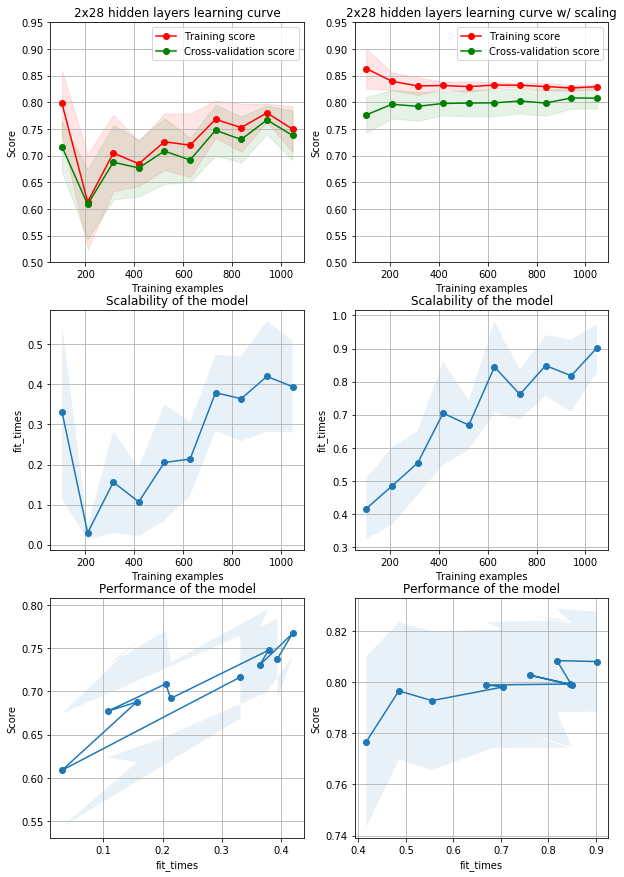
\includegraphics[width=\textwidth,height=\textheight,keepaspectratio]{plot-nn-learningcurve.png}
	\caption{Accuracy is the score considered. Running on the chosen model the learning curve, scalability and performance. Same data, left side is not scaled. Scaling the values improves the accuracy, while increasing the fit\_time. }
	\label{figure:graph-nn-scalevsnoscale}
\end{figure}




\section{Decision trees and random forest}
\subsection{Introduction: Decision Trees}
A decision tree builds upon iteratively asking questions to partition data.
Our aim is to increase the predictiveness of the model as much as possible at each partitioning so that the model keeps gaining information about the dataset.
There are two ways to measure the quality of a split:
\begin{enumerate}
	\item Gini-Index: The measure is about the impurity of a node. The aim is to reduce the impurity (reduce randomness) of data to achieve correct classification (labeling).
	\item Information Gain (Entropy):
	The information gain is the difference between entropy before and after the split.
	When splitting decision trees try to be more predictive, less impure and reduce entropy. Entropy is a measure of uncertainty or randomness. The more randomness a variable (feature) has, the higher the entropy is.  
\end{enumerate}

\subsection{Procedure: Decision Trees}
M5PrimeLab Octave toolbox has been chosen.
\begin{enumerate}  
	\item The model tree is build with suggested parameters. Customization of parameters has been necessary to achieve a printable plot. For example, pruning and smoothing factor are not applied to get better performance in tree construction.
	\item Different values for K are tried to run Cross Validation. Various experiments has showed K=10 is ideal for best trade-off between metrics and algorithm running times. The collected measures are MAE, MSE, RMSE, RRMSE, R2, nRules, nVars (table \ref{tab:CV-ModelTree}).
	\item The regression tree is build with suggested parameters. Also in this case parameters has to be adjusted for best plotting. The main difference to model tree is that the leaf nodes contain response values instead of models. As for the model tree K=10 leads to the best results in the Cross Validation folding technique. The resulting measures are very similar to those ot the model tree (table \ref{tab:CV-RegressionTree}).
	\item The model tree prediction has been calculated (table \ref{tab:Result-Prediction}). A further important insight is the input variable contributions (table \ref{tab:Vars-Contribution}).  The top three variables influencing the model are: Title (Mr.), Pclass 3 (lower class) and Sibsp (number of siblings/spouses).
	\item The decision rules are extracted from the model tree. For curiosity the 10-fold Cross Validation technique is applied on the rules configuration (table \ref{tab:CV-Rules}) to compare the measures with those of the trees (model and regression). The Mean Square Error (MSE) is slightly higher although the number of rules used are more than halved.
\end{enumerate}

\subsection{Results: Decision Trees}
The M5 algorithm generated 163 different rules using 13 variables.
\break After 10-fold Cross Validation with 14 variables used the number of rules lowered to 71.

\bigskip
Following Measures are collected:
\begin{itemize}
	\item MAE (Mean Absolute Error)
	\item MSE (Mean Squared Error)
	\item RMSE (Root Mean Squared Error)
	\item RRMSE (Relative Root Mean Squared Error)
	\item R2 (Coefficient of Determination)
	\item nRules (Mean Number of Rules)
	\item nVars (Mean Number of Variables)
\end{itemize}

\begin{table}[H]
	\centering
	\caption{10-fold Cross Validation on Model Tree}
	\label{tab:CV-ModelTree}
	\begin{tabular}{|l|l|}
		\hline
		\textbf{Measure} & \textbf{Value} \\ \hline
		MAE       		& 0.23878 \\ \hline
		MSE       		& 0.18681 \\ \hline
		RMSE       		& 0.43123 \\ \hline
		RRMSE       	& 0.88923 \\ \hline
		R2       		& 0.20563 \\ \hline
		nRules       	& 146.60  \\ \hline
		nVars       	& 12.500  \\ \hline
	\end{tabular}
\end{table}

\begin{table}[H]
	\centering
	\caption{10-fold Cross Validation on Regression Tree}
	\label{tab:CV-RegressionTree}
	\begin{tabular}{|l|l|}
		\hline
		\textbf{Measure} 	& \textbf{Value} \\ \hline
		MAE       			& 0.23908 		 \\ \hline
		MSE       			& 0.18327 		 \\ \hline
		RMSE       			& 0.42722		 \\ \hline
		RRMSE       		& 0.88093 	  	 \\ \hline
		R2       			& 0.22085  	 	 \\ \hline
		nRules       		& 148.10   		 \\ \hline
		nVars       		& 12.500   		 \\ \hline
	\end{tabular}
\end{table}

\begin{table}[H]
	\centering
	\caption{Result Prediction}
	\label{tab:Result-Prediction}
	\begin{tabular}{|l|l|}
		\hline
		\textbf{Measure}    & \textbf{Value} \\ \hline
		Prediction       	& 1.000000 	  	 \\ \hline
		Training set mean   & 0.381971 	  	 \\ \hline
	\end{tabular}
\end{table}

\begin{table}[H]
	\centering
	\caption{Input variable contributions}
	\label{tab:Vars-Contribution}
	\begin{tabular}{|l|l|}
		\hline
		\textbf{Variable}   & \textbf{Contribution}	\\ \hline
		Title-Mr. (x17)	    & 0.301000 				\\ \hline
		Pclass-3 (x26)	    & 0.196754 				\\ \hline
		Sibsp (x2)	       	& 0.090909 				\\ \hline
		Title-Rev (x20)	    & 0.024869				\\ \hline
		Gender (x5)	       	& 0.022520 				\\ \hline
		Fare (x4)	       	& -0.018023 			\\ \hline
	\end{tabular}
\end{table}

\begin{table}[H]
	\centering
	\caption{10-fold Cross Validation on Rules configuration}
	\label{tab:CV-Rules}
	\begin{tabular}{|l|l|}
		\hline
		\textbf{Measure} 	& \textbf{Value} \\ \hline
		MAE       			& 0.25774 		 \\ \hline
		MSE       			& 0.18812 		 \\ \hline
		RMSE       			& 0.43288		 \\ \hline
		RRMSE       		& 0.89289 	  	 \\ \hline
		R2       			& 0.19922  	 	 \\ \hline
		nRules       		& 67.100   		 \\ \hline
		nVars       		& 14.700   		 \\ \hline
	\end{tabular}
\end{table}
\newpage
\vfill
\begin{sidewaysfigure}[h]
	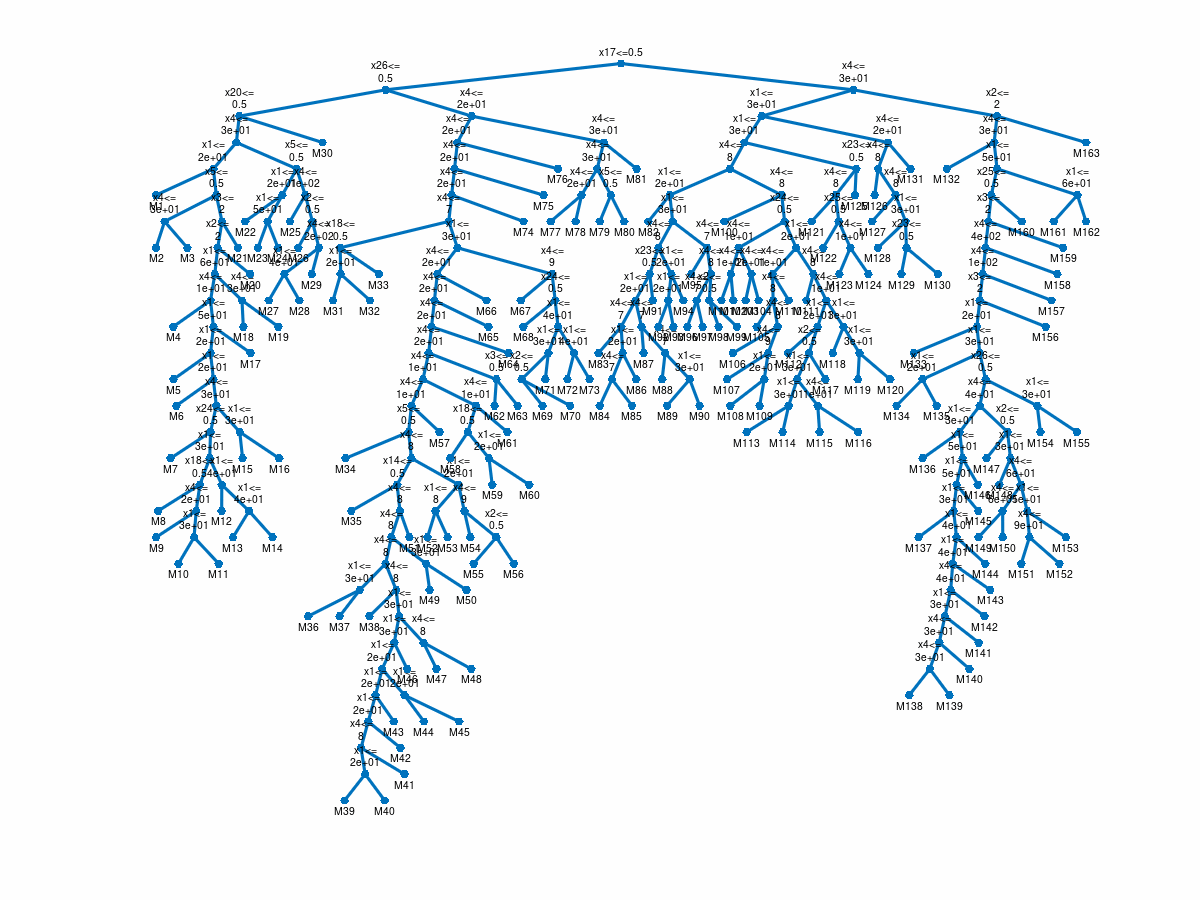
\includegraphics[width=\textwidth,height=\textheight,keepaspectratio]{model_tree.png}
	\caption{Model Tree}
\end{sidewaysfigure}	
\begin{sidewaysfigure}[h]
	\centering
	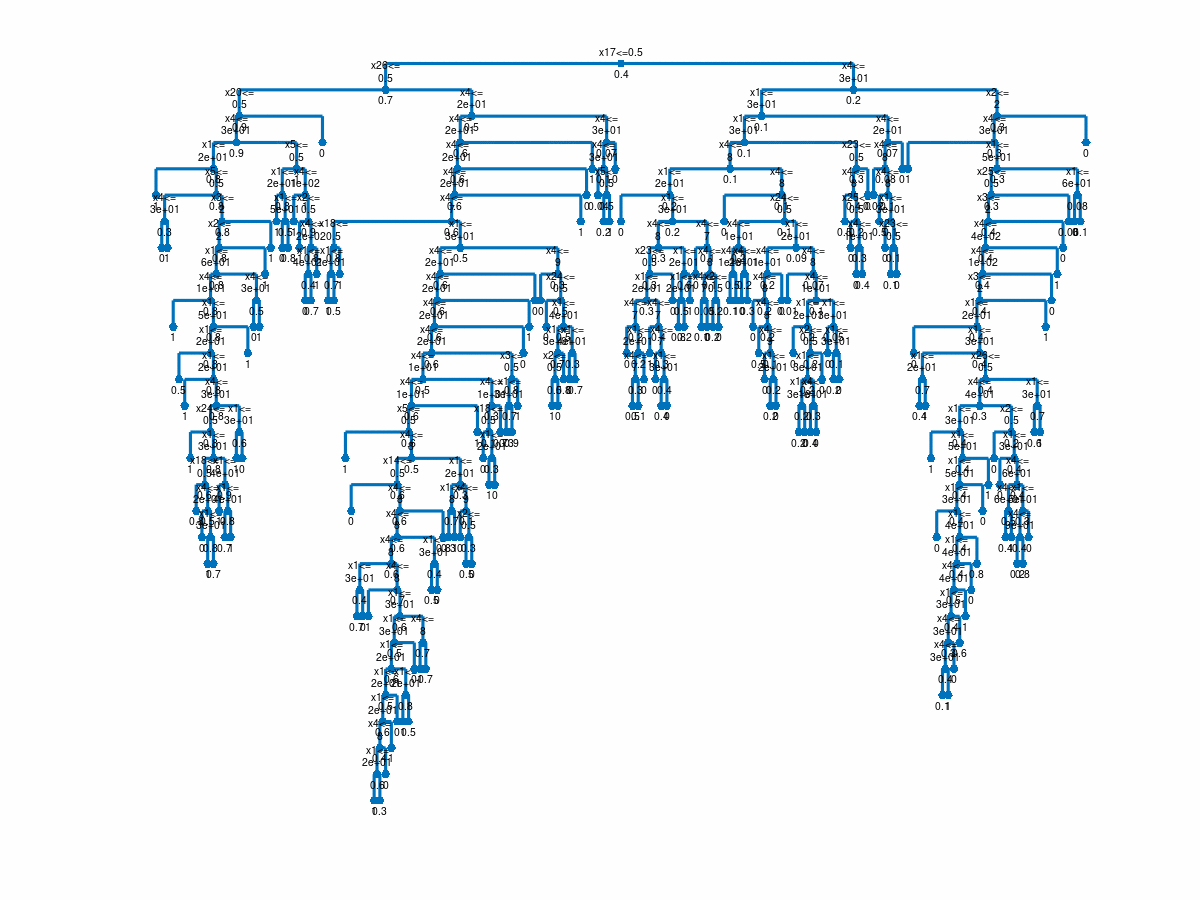
\includegraphics[width=\textwidth,height=\textheight,keepaspectratio]{regression_tree.png}
	\caption{Regression Tree}
\end{sidewaysfigure}
\vfill
\clearpage

\subsection{Outcome explanation}
Decision trees do not need normalization or feature scaling to work well. They are suitable for mixed feature data types and the result interpretation of small depth trees is easy. However, they tend to overfit data (high depth trees) and cause higher variance in the model. The Cross Validation technique lowered the decision rules from 163 to 71. This is linked with the fact that K subsets has been used to train the model instead of using the complete dataset.

\subsection{Introduction: Random Forest}
Random forest is an ensemble of many decision trees. Random forests are built using a method called bagging in which each decision tree is used as parallel estimator.
Random forests reduce the risk of overfitting and accuracy is much higher than a single decision tree. Furthermore, decision trees in a random forest run in parallel so that the time does not become a bottleneck but performance is required.

\subsection{Procedure: Random Forest}
M5PrimeLab Octave toolbox has been chosen.
\begin{enumerate}  
	\item The tree forest also called ensemble is build with suggested parameters. Customization of parameters has been necessary to lower as much as possible the Mean Square Error (MSE) (figure \ref{fig:MSE-general}). Different features subsets lead to various error rates (figure \ref{fig:MSE}). The lowest error rate is obtained using 8 features. The number utilized trees is set to 50 for obtaining the best trade-off between metrics and running times. Growing big ensembles is very expensive. For this reason higher values of 50 are not taken into consideration. 
	\item The variable importance (influence) is plotted (figure \ref{fig:Var-Importance}). In an ensembles, in contrast to the single decision tree, a greater combination of features contribute to the result because the sampling with replacement mechanism is used.
	\item Cross Validation folding technique is used to evaluate the predictive performance of the forest. The best MSE is obtained with K=10. Higher values cause a relevant growth in the algorithm running times. As seen in figure \ref{fig:CV} Cross validation MSE is lower than the Out-of-bag MSE. Out-of-bag MSE is suitable for low datasets where a splitting is not possible.
\end{enumerate}

\subsection{Results: Random Forest}
An ensemble is grown with 50 trees using Random Forest. As illustrated the lowest Mean Square Error (MSE) is achieved with 50 trees. The MSE of random forest is lower than the one of the single decision tree. From around 18\% it has lowered to around 14\%. That proves Random Forest technique is a more powerful than building single decision trees. Although, more computational power is required.

\begin{figure}[H]
	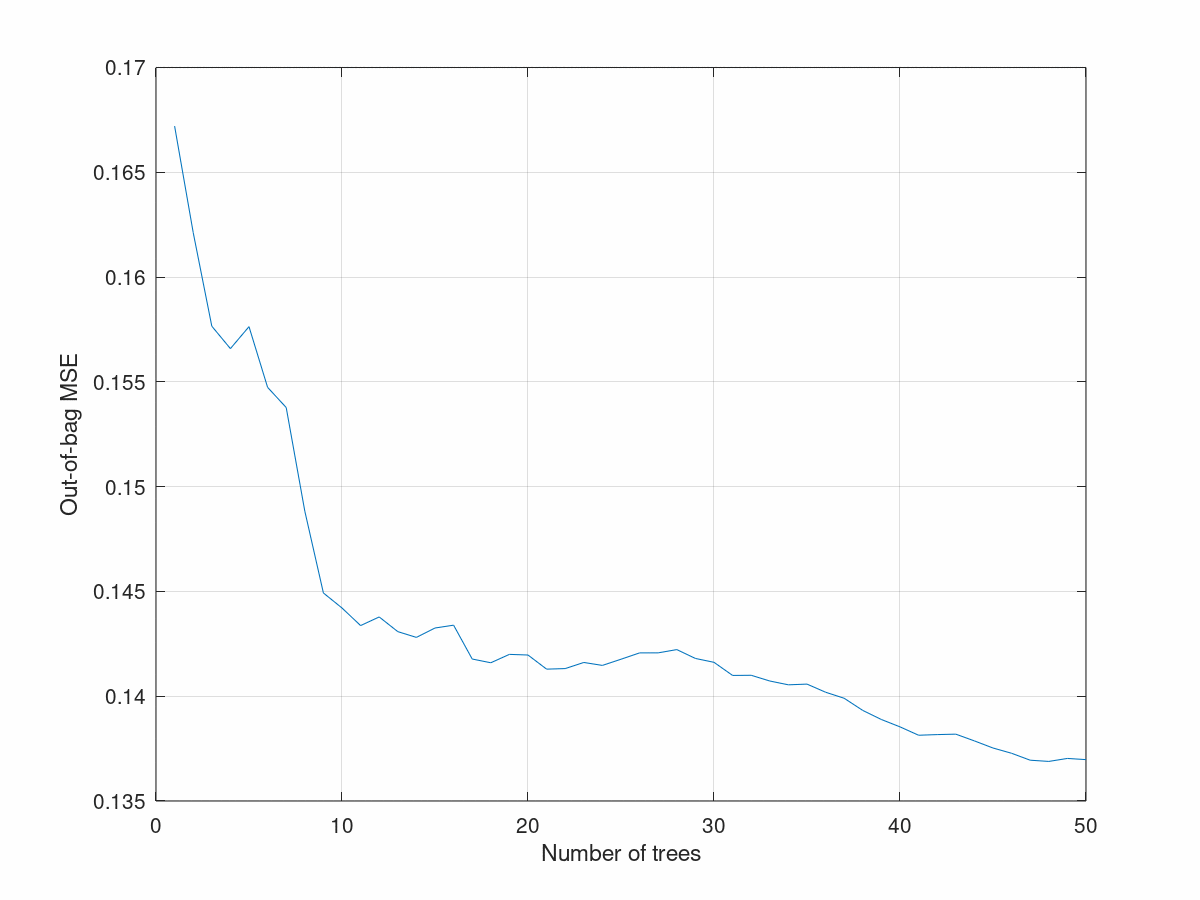
\includegraphics[width=\textwidth,height=\textheight,keepaspectratio]{mse.png}
	\caption{MSE}
	\label{fig:MSE-general}
\end{figure}

\begin{figure}[H]
	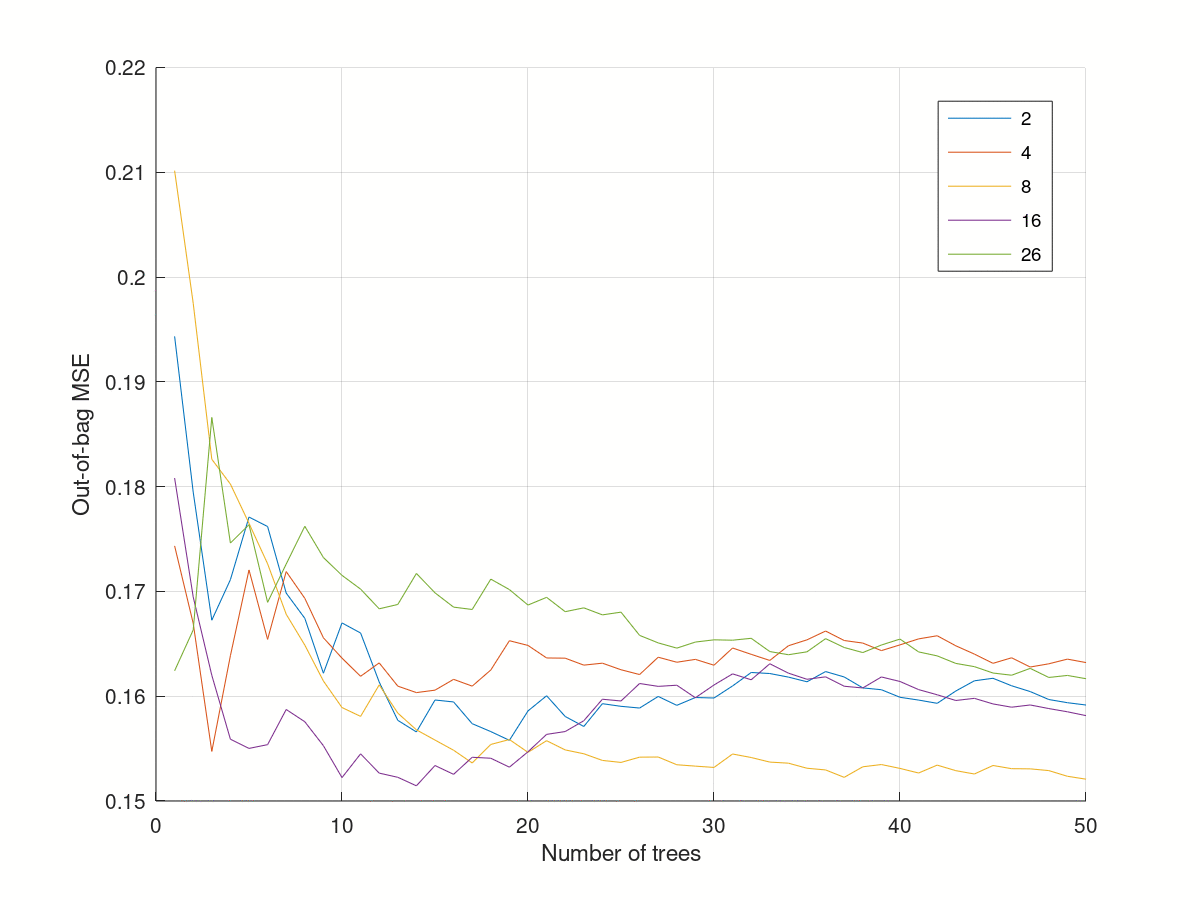
\includegraphics[width=\textwidth,height=\textheight,keepaspectratio]{mse_rf.png}
	\caption{MSE Random Forest}
	\label{fig:MSE}
\end{figure}

\begin{figure}[H]
	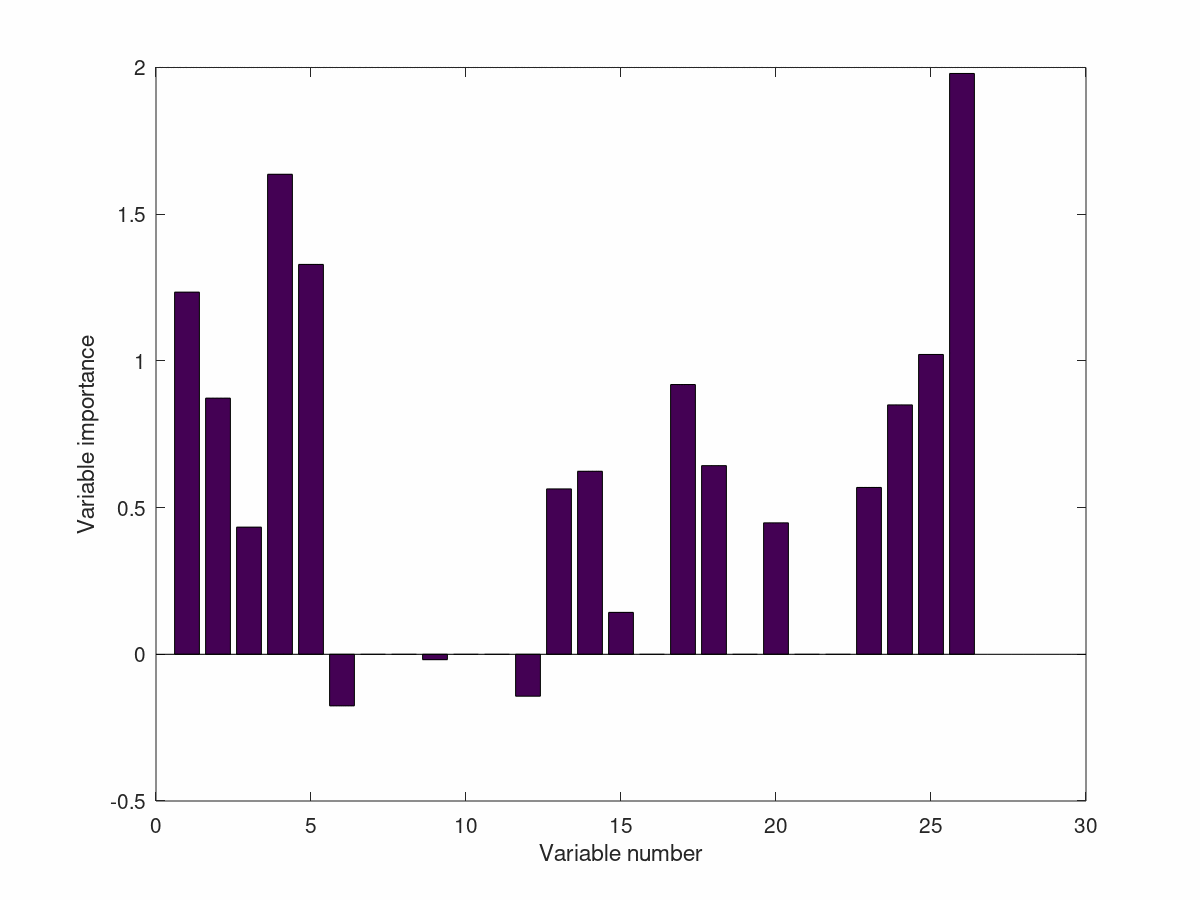
\includegraphics[width=\textwidth,height=\textheight,keepaspectratio]{var_importance.png}
	\caption{Variable Importance}
	\label{fig:Var-Importance}
\end{figure}

\begin{figure}[H]
	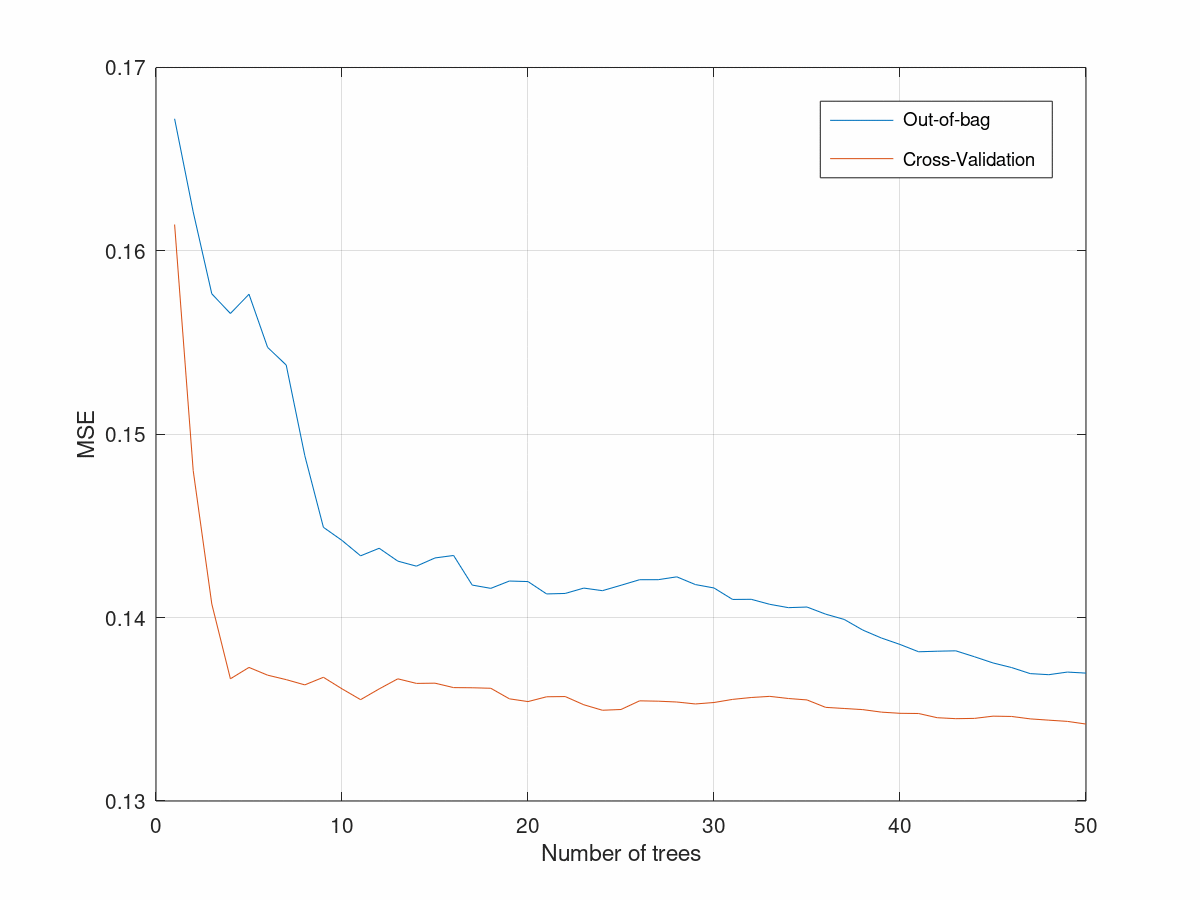
\includegraphics[width=\textwidth,height=\textheight,keepaspectratio]{bag_vs_cv.png}
	\caption{Cross Validation vs Out-of-bag MSE}
	\label{fig:CV}
\end{figure}
	
\subsection{Outcome explanation}
Random forests solve the overfitting problem due to the averaged result extracted from the tree ensemble. However, with high-dimensional data scalability problems arise.
The usage of an ensemble of size 50 gave the best results. With 100 and more trees the results do not change expect the running times due to the greater amount of trees to build. The fact that 8 features in combination with 50 trees achieve the lowest error rate is because the dataset is composed by features of different importance which tend to influence differently the classifier results. Also correlations between features play a crucial role in this context.

\section{Naive Bayes Classifier}
A Naive Bayes classifier is a probabilistic machine learning model that’s used for classification task. The classifier is based on the probabilistic Bayes theorem.
\begin{equation}
\label{eq:bayes-theorem}
P(A|B) = \frac{P(B|A) P(A)}{P(B)}
\end{equation}
Using Bayes theorem, we can find the probability of A happening, given that B has occurred. Here, B is the evidence and A is the hypothesis. The assumption made here is that the predictors/features are independent. That means presence of one particular feature does not affect the other one (naive feature).

\bigskip
Following types of classifier exist:
\begin{itemize}
	\item Multinomial Naive Bayes: for document classification
	\item Bernoulli Naive Bayes: similar to Multinomial using boolean variables
	\item Gaussian Naive Bayes: for datasets with continuous features
\end{itemize}

\subsection{Procedure}
Python Scikit-learn library has been chosen.
\begin{enumerate}  
	\item The Pearson correlation coefficient (PCC) on each pair of features is plotted to inspect the correlation between features (heat-map \ref{fig:PCC}). Naive Bayes classifier requires independent features to get the best results.
	\item The three types of Naive Bayes classifier (Gaussian, Bernoulli, Multinomial) are used on the test set (30\% of dataset) to inspect the incorrect prediction results (table \ref{tab:result-comparison}). Bernoulli Naive Bayes achieved the lowest error rate.
	\item The model metrics using the Gaussian Naive Bayes (table \ref{tab:Gaussian-metrics}) and Bernoulli Naive Bayes (table \ref{tab:Bernoulli-metrics}) are calculated and the probability of each class (dead or survived) is predicted (table \ref{tab:result-comparison}). Gaussian Naive Bayes achieved the better scores.
	\item For a better understanding the learning curves for Gaussian classifier (figure \ref{fig:Gaussian-curve}) and Bernoulli classifier (figure \ref{fig:Bernoulli-curve}) are plotted. Bernoulli classifier achieves more stable scores and the scaling does not influence the performance. Gaussian classifier suffers from scaling.
\end{enumerate}


\subsection{Results}
\begin{figure}[H]
	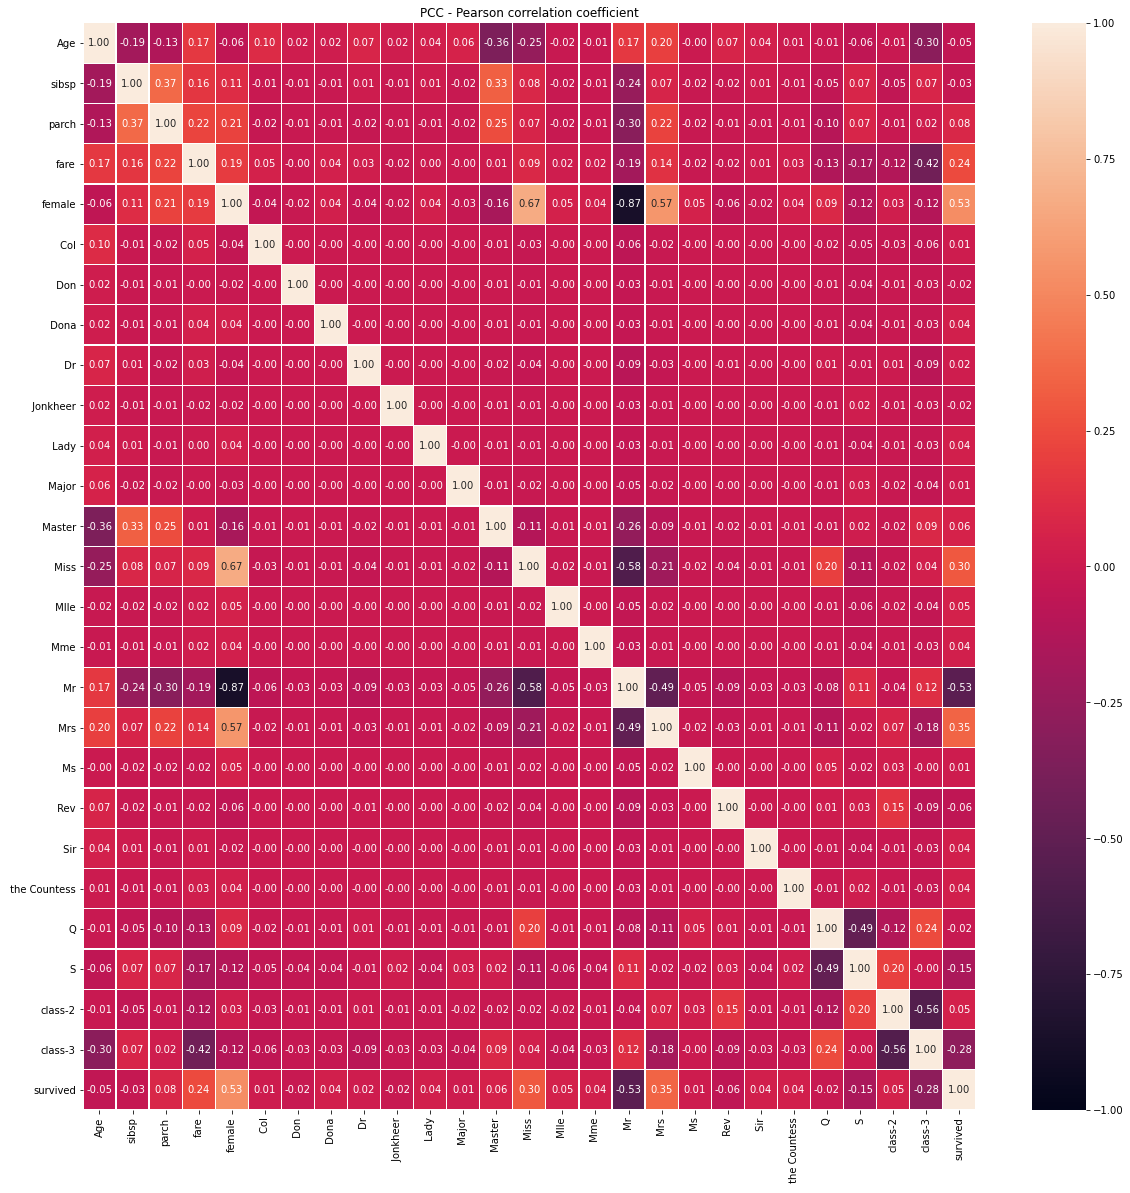
\includegraphics[width=\textwidth,height=\textheight,keepaspectratio]{heat_map.png}
	\caption{PCC - Pearson correlation coefficient}
	\label{fig:PCC}
\end{figure}

\begin{table}[H]
	\centering
	\caption{Results comparison using 432 test records)}
	\label{tab:result-comparison}
	\begin{tabular}{|l|l|l|}
		\hline
		\textbf{Measure} & \textbf{correct} & \textbf{incorrect} \\ \hline
		Gaussian Naive Bayes       	 & 288    & 144 \\ \hline
		Multinomial Naive Bayes      & 302    & 130 \\ \hline
		Bernoulli Naive Bayes    	 & 322    & 110 \\ \hline
	\end{tabular}
\end{table}

\begin{table}[H]
	\centering
	\caption{Model metrics - Gaussian Naive Bayes}
	\label{tab:Gaussian-metrics}
	\begin{tabular}{|l|l|l|}
		\hline
		\textbf{Measure} & \textbf{Train} & \textbf{Validation} \\ \hline
		Accuracy       	 & 0.80    & 0.84 \\ \hline
		Recall    		 & 0.72    & 0.82 \\ \hline
		Precision    	 & 0.74    & 0.75 \\ \hline
	\end{tabular}
\end{table}

\begin{table}[H]
	\centering
	\caption{Model metrics - Bernoulli Naive Bayes}
	\label{tab:Bernoulli-metrics}
	\begin{tabular}{|l|l|l|}
		\hline
		\textbf{Measure} & \textbf{Train} & \textbf{Validation} \\ \hline
		Accuracy       	 & 0.79    & 0.81 \\ \hline
		Recall    		 & 0.71    & 0.79 \\ \hline
		Precision    	 & 0.73    & 0.74 \\ \hline
	\end{tabular}
\end{table}

\begin{table}[H]
	\centering
	\caption{Probability of each class}
	\label{tab:NB-probabilities}
	\begin{tabular}{|l|l|}
		\hline
		\textbf{Measure} & \textbf{Value} \\ \hline
		Survive  = 0     & 0.62    \\ \hline
		Survive  = 1     & 0.38   \\ \hline
	\end{tabular}
\end{table}

\begin{figure}[H]
	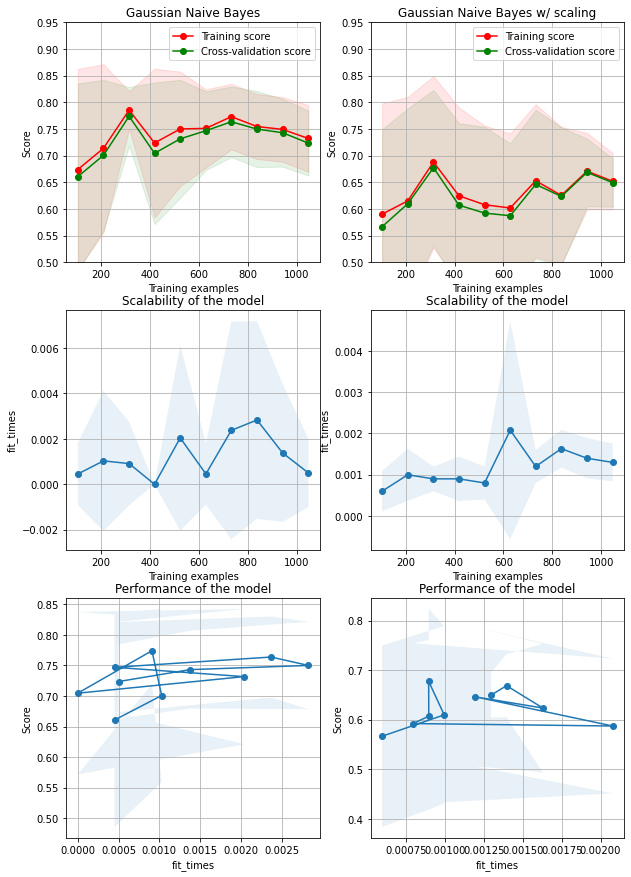
\includegraphics[width=\textwidth,height=\textheight,keepaspectratio]{gaussianNB_curve.png}
	\caption{Gaussian Naive Bayes: the learning curve, scalability and performance. Right part is with scaled data.}
	\label{fig:Gaussian-curve}
\end{figure}

\begin{figure}[H]
	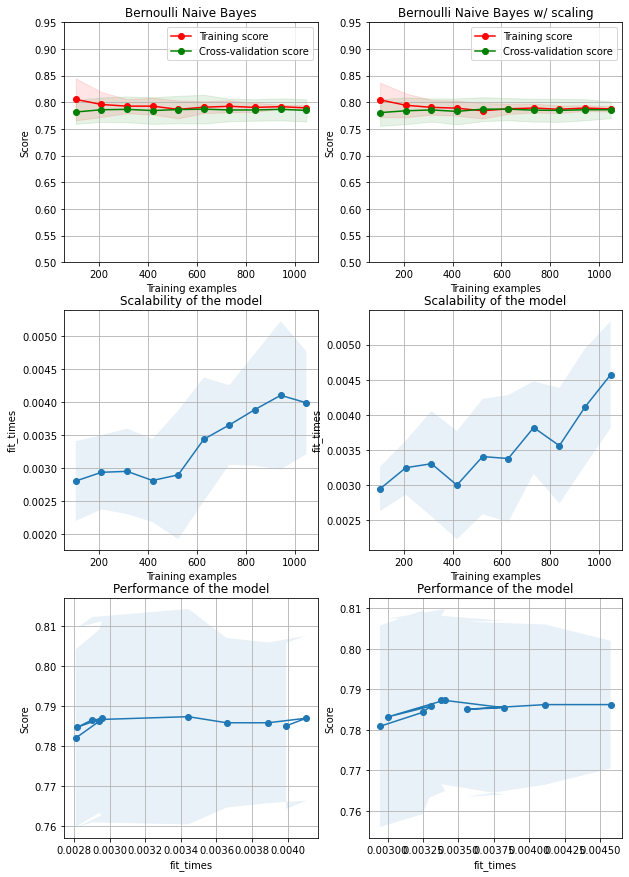
\includegraphics[width=\textwidth,height=\textheight,keepaspectratio]{bernoulliNB_curve.png}
	\caption{Bernoulli Naive Bayes: the learning curve, scalability and performance. Right part is with scaled data.}
	\label{fig:Bernoulli-curve}
\end{figure}

\subsection{Outcome explanation}
Naive Bayes is easy and fast to implement. The algorithm works well in most of the cases because the crux is the calculation of probabilities. However, the correlation between features alters the probability calculation. Therefore, the best metrics are only achieved providing datasets with as much as possible independent features. The better scoring results of Bernoulli classifier is based on the massive presence of boolean variables ("dummy variables").

\section{Conclusion}
Machine learning is a constantly evolving broad and interesting topic.
\break This project gave us the possibility to experiment with Supervised Learning algorithms.
As mentioned in the lectures, there is no silver bullet that can be applied to every problem. Every algorithm has its characteristics and relative drawbacks. Real-World experice seems to be required to choose the best fitting methodology a priori.
The project was stimulating, so much that it opnened up the possibility of partecipating in some data science challenges available in kaggle.com.
\end{document}

